% Options for packages loaded elsewhere
\PassOptionsToPackage{unicode}{hyperref}
\PassOptionsToPackage{hyphens}{url}
\PassOptionsToPackage{dvipsnames,svgnames,x11names}{xcolor}
%
\documentclass[
]{article}

\usepackage{amsmath,amssymb}
\usepackage{iftex}
\ifPDFTeX
  \usepackage[T1]{fontenc}
  \usepackage[utf8]{inputenc}
  \usepackage{textcomp} % provide euro and other symbols
\else % if luatex or xetex
  \usepackage{unicode-math}
  \defaultfontfeatures{Scale=MatchLowercase}
  \defaultfontfeatures[\rmfamily]{Ligatures=TeX,Scale=1}
\fi
\usepackage{lmodern}
\ifPDFTeX\else  
    % xetex/luatex font selection
  \setmainfont[]{Latin Modern Roman}
  \setmathfont[]{Latin Modern Math}
\fi
% Use upquote if available, for straight quotes in verbatim environments
\IfFileExists{upquote.sty}{\usepackage{upquote}}{}
\IfFileExists{microtype.sty}{% use microtype if available
  \usepackage[]{microtype}
  \UseMicrotypeSet[protrusion]{basicmath} % disable protrusion for tt fonts
}{}
\makeatletter
\@ifundefined{KOMAClassName}{% if non-KOMA class
  \IfFileExists{parskip.sty}{%
    \usepackage{parskip}
  }{% else
    \setlength{\parindent}{0pt}
    \setlength{\parskip}{6pt plus 2pt minus 1pt}}
}{% if KOMA class
  \KOMAoptions{parskip=half}}
\makeatother
\usepackage{xcolor}
\setlength{\emergencystretch}{3em} % prevent overfull lines
\setcounter{secnumdepth}{5}
% Make \paragraph and \subparagraph free-standing
\ifx\paragraph\undefined\else
  \let\oldparagraph\paragraph
  \renewcommand{\paragraph}[1]{\oldparagraph{#1}\mbox{}}
\fi
\ifx\subparagraph\undefined\else
  \let\oldsubparagraph\subparagraph
  \renewcommand{\subparagraph}[1]{\oldsubparagraph{#1}\mbox{}}
\fi


\providecommand{\tightlist}{%
  \setlength{\itemsep}{0pt}\setlength{\parskip}{0pt}}\usepackage{longtable,booktabs,array}
\usepackage{calc} % for calculating minipage widths
% Correct order of tables after \paragraph or \subparagraph
\usepackage{etoolbox}
\makeatletter
\patchcmd\longtable{\par}{\if@noskipsec\mbox{}\fi\par}{}{}
\makeatother
% Allow footnotes in longtable head/foot
\IfFileExists{footnotehyper.sty}{\usepackage{footnotehyper}}{\usepackage{footnote}}
\makesavenoteenv{longtable}
\usepackage{graphicx}
\makeatletter
\def\maxwidth{\ifdim\Gin@nat@width>\linewidth\linewidth\else\Gin@nat@width\fi}
\def\maxheight{\ifdim\Gin@nat@height>\textheight\textheight\else\Gin@nat@height\fi}
\makeatother
% Scale images if necessary, so that they will not overflow the page
% margins by default, and it is still possible to overwrite the defaults
% using explicit options in \includegraphics[width, height, ...]{}
\setkeys{Gin}{width=\maxwidth,height=\maxheight,keepaspectratio}
% Set default figure placement to htbp
\makeatletter
\def\fps@figure{htbp}
\makeatother
\newlength{\cslhangindent}
\setlength{\cslhangindent}{1.5em}
\newlength{\csllabelwidth}
\setlength{\csllabelwidth}{3em}
\newlength{\cslentryspacingunit} % times entry-spacing
\setlength{\cslentryspacingunit}{\parskip}
\newenvironment{CSLReferences}[2] % #1 hanging-ident, #2 entry spacing
 {% don't indent paragraphs
  \setlength{\parindent}{0pt}
  % turn on hanging indent if param 1 is 1
  \ifodd #1
  \let\oldpar\par
  \def\par{\hangindent=\cslhangindent\oldpar}
  \fi
  % set entry spacing
  \setlength{\parskip}{#2\cslentryspacingunit}
 }%
 {}
\usepackage{calc}
\newcommand{\CSLBlock}[1]{#1\hfill\break}
\newcommand{\CSLLeftMargin}[1]{\parbox[t]{\csllabelwidth}{#1}}
\newcommand{\CSLRightInline}[1]{\parbox[t]{\linewidth - \csllabelwidth}{#1}\break}
\newcommand{\CSLIndent}[1]{\hspace{\cslhangindent}#1}


\newcommand{\Xobs}{\mathbf{X}_{\text{obs}}}
\newcommand{\Xsyn}{\mathbf{X}_{\text{syn}}}
\newcommand{\dist}{\mathcal{P}}
\newcommand{\pobs}{p_{\text{obs}}}
\newcommand{\psyn}{p_{\text{syn}}}
\newcommand{\nobs}{n_{\text{obs}}}
\newcommand{\nsyn}{n_{\text{syn}}}
\newcommand{\bx}{\mathbf{x}}
\usepackage{arxiv}
\usepackage{orcidlink}
\usepackage{amsmath}
\usepackage[T1]{fontenc}
\makeatletter
\makeatother
\makeatletter
\makeatother
\makeatletter
\@ifpackageloaded{caption}{}{\usepackage{caption}}
\AtBeginDocument{%
\ifdefined\contentsname
  \renewcommand*\contentsname{Table of contents}
\else
  \newcommand\contentsname{Table of contents}
\fi
\ifdefined\listfigurename
  \renewcommand*\listfigurename{List of Figures}
\else
  \newcommand\listfigurename{List of Figures}
\fi
\ifdefined\listtablename
  \renewcommand*\listtablename{List of Tables}
\else
  \newcommand\listtablename{List of Tables}
\fi
\ifdefined\figurename
  \renewcommand*\figurename{Figure}
\else
  \newcommand\figurename{Figure}
\fi
\ifdefined\tablename
  \renewcommand*\tablename{Table}
\else
  \newcommand\tablename{Table}
\fi
}
\@ifpackageloaded{float}{}{\usepackage{float}}
\floatstyle{ruled}
\@ifundefined{c@chapter}{\newfloat{codelisting}{h}{lop}}{\newfloat{codelisting}{h}{lop}[chapter]}
\floatname{codelisting}{Listing}
\newcommand*\listoflistings{\listof{codelisting}{List of Listings}}
\makeatother
\makeatletter
\@ifpackageloaded{caption}{}{\usepackage{caption}}
\@ifpackageloaded{subcaption}{}{\usepackage{subcaption}}
\makeatother
\makeatletter
\@ifpackageloaded{tcolorbox}{}{\usepackage[skins,breakable]{tcolorbox}}
\makeatother
\makeatletter
\@ifundefined{shadecolor}{\definecolor{shadecolor}{rgb}{.97, .97, .97}}
\makeatother
\makeatletter
\makeatother
\makeatletter
\makeatother
\ifLuaTeX
  \usepackage{selnolig}  % disable illegal ligatures
\fi
\IfFileExists{bookmark.sty}{\usepackage{bookmark}}{\usepackage{hyperref}}
\IfFileExists{xurl.sty}{\usepackage{xurl}}{} % add URL line breaks if available
\urlstyle{same} % disable monospaced font for URLs
\hypersetup{
  pdftitle={A density ratio framework for evaluating the utility of synthetic data},
  pdfauthor={Thom Benjamin Volker; Peter-Paul de Wolf; Erik-Jan van Kesteren},
  pdfkeywords={synthetic data, utility, density ratio, privacy,
disclosure limitation},
  colorlinks=true,
  linkcolor={blue},
  filecolor={Maroon},
  citecolor={Blue},
  urlcolor={Blue},
  pdfcreator={LaTeX via pandoc}}

\usepackage{setspace}
\doublespacing
\newcommand{\runninghead}{A Preprint }
\renewcommand{\runninghead}{Density ratios for utility }
\title{A density ratio framework for evaluating the utility of synthetic
data}
\def\asep{\\\\\\ } % default: all authors on same column
\def\asep{\And }
\author{\textbf{Thom Benjamin
Volker}~\orcidlink{0000-0002-2408-7820}\\Methodology and Statistics
\textbar{} Methodology\\Utrecht University \textbar{} Statistics
Netherlands\\Utrecht,\ 3584CH\\\href{mailto:t.b.volker@uu.nl}{t.b.volker@uu.nl}\asep\textbf{Peter-Paul
de Wolf}\\Methodology\\Statistics Netherlands\\The
Hague,\ 2490HA\\\href{mailto:pp.dewolf@cbs.nl}{pp.dewolf@cbs.nl}\asep\textbf{Erik-Jan
van Kesteren}\\Methodology and Statistics\\Utrecht
University\\Utrecht,\ 3584CH\\\href{mailto:e.vankesteren1@uu.nl}{e.vankesteren1@uu.nl}}
\date{}
\begin{document}
\maketitle
\begin{abstract}
TODO TODO TODO TODO TODO TODO TODO TODO TODO TODO TODO TODO TODO TODO
TODO TODO TODO TODO TODO TODO TODO TODO TODO TODO TODO TODO TODO TODO
TODO TODO TODO TODO TODO TODO TODO TODO TODO TODO TODO TODO TODO TODO
TODO TODO TODO TODO TODO TODO TODO TODO TODO TODO TODO TODO TODO TODO
TODO TODO TODO TODO TODO TODO TODO TODO TODO TODO TODO TODO TODO TODO
TODO TODO TODO TODO TODO TODO TODO TODO TODO TODO TODO TODO TODO TODO
TODO TODO TODO TODO TODO TODO TODO TODO TODO TODO TODO TODO TODO TODO
TODO TODO TODO TODO TODO TODO TODO TODO TODO TODO TODO TODO TODO TODO
TODO TODO TODO TODO TODO TODO TODO TODO TODO TODO TODO TODO TODO TODO
TODO TODO TODO TODO TODO TODO TODO TODO TODO TODO TODO TODO TODO TODO
TODO TODO TODO TODO TODO TODO TODO TODO TODO TODO TODO
\end{abstract}
{\bfseries \emph Keywords}
\def\sep{\textbullet\ }
synthetic data, utility, density ratio, privacy, disclosure
limitation \sep 
synthetic data, utility, density ratio, privacy, disclosure limitation

\ifdefined\Shaded\renewenvironment{Shaded}{\begin{tcolorbox}[boxrule=0pt, interior hidden, frame hidden, borderline west={3pt}{0pt}{shadecolor}, sharp corners, breakable, enhanced]}{\end{tcolorbox}}\fi

\hypertarget{introduction}{%
\section{Introduction}\label{introduction}}

Openly accessible research data accelerates scientific progress
tremendously. Open data allows third-party researchers to answer
research questions with already collected data, freeing up resources
that would otherwise be devoted to data collection
(\protect\hyperlink{ref-ramachandran_open_2021}{Ramachandran, Bugbee,
and Murphy 2021}). Sharing data in combination with code allows others
to validate research findings and build upon the work
(\protect\hyperlink{ref-obels_analysis_2020}{Obels et al. 2020};
\protect\hyperlink{ref-crosas_automating_2015}{Crosas et al. 2015}).
Students can benefit from open data, as it fosters education with
realistic data (\protect\hyperlink{ref-atenas_open_2015}{Atenas,
Havemann, and Priego 2015}), as well as the general public, through
stimulating citizen science projects
(\protect\hyperlink{ref-newman_future_2012}{Newman et al. 2012}).
However, making data openly available is often (rightfully) hampered by
official legislation, like the General Data Protection Regulation (GDPR;
\protect\hyperlink{ref-gdpr}{European Parliament and Council of the
European Union 2016}), and general privacy concerns. In the worst case,
sharing data may cause harm to individuals or organizations, which may
withhold these entities from participating in future research. These
privacy constraints have been named among the biggest hurdles in the
advancement of computational social science
(\protect\hyperlink{ref-lazer_css_2009}{Lazer et al. 2009}), and among
top reasons for companies to not share their data with researchers
(\protect\hyperlink{ref-fpf_2017}{Future of Privacy Forum 2017}).

Multiple approaches exist to balance the benefits of open data with
potential privacy risks. Traditionally, data providers employed a suite
of different disclosure limitation techniques before sharing the data,
such as top-coding, record-swapping or adding noise (e.g.,
\protect\hyperlink{ref-hundepool_disclosure_2012}{Hundepool et al.
2012}; \protect\hyperlink{ref-willenborg_elements_2001}{Willenborg and
De Waal 2001}). More recently, synthetic data has gained traction as a
means to disseminate private data
(\protect\hyperlink{ref-SIPP_Beta_2006}{Abowd, Stinson, and Benedetto
2006}; \protect\hyperlink{ref-hawala_synthetic_2008}{Hawala 2008};
\protect\hyperlink{ref-drechsler2012}{Drechsler 2012};
\protect\hyperlink{ref-vandewiel2023}{van de Wiel et al. 2023};
\protect\hyperlink{ref-obermeyer2019}{Obermeyer et al. 2019};
\protect\hyperlink{ref-zettler2021}{Zettler et al. 2021}), although the
conceptual framework traces back to the previous century
(\protect\hyperlink{ref-little_statistical_1993}{Little 1993};
\protect\hyperlink{ref-rubin_statistical_1993}{Rubin 1993}). Simply put,
the idea of synthetic data is to replace some, or all, of the observed
values in a data set by synthetic values that are generated from some
model (e.g., \protect\hyperlink{ref-drechsler2011synthetic}{Drechsler
2011}). If only some values are replaced, disclosure risks can be
reduced because the sensitive or identifying values do not correspond to
their true values anymore. If all values are replaced, there is also no
one-to-one mapping between the original and the synthetic data, further
reducing the disclosure risk. However, an increase in privacy typically
comes at the cost of a decrease in utility. As more of the data is
altered, the quality of the released data becomes more sensitive to the
suitability of the generative model. Regardless of the approach to
disclosure limitation, if the technique used to generate or alter the
data does not align with the intricacies of the problem at hand, the
utility of the released data will be further reduced than necessary.

Given that all disclosure limitation techniques reduce the utility of
the data, the challenge that arises is how to determine whether the
released data still has acceptable utility. Alternatively, one might
consider different disclosure limitation techniques that all satisfy the
defined privacy restrictions, and employ the one which yields data with
the highest utility. That is, given a set of methods that all meet the
privacy restrictions, one may aim to maximize the utility of the
released data. Both strategies require a reliable and encompassing
measure of data utility that allows to evaluate the quality of the
released data, and that allows to compare different disclosure
limitation techniques and/or synthesis models in terms of utility.
Moreover, adequate utility measures often guide the synthesis process,
by providing detailed feedback on important discrepancies between the
original and synthetic data. Lastly, good utility measures help the data
user in determining what the synthetic data can and cannot be used for.

In the synthetic data field, three classes of utility measures have been
distinguished (see \protect\hyperlink{ref-drechsler2023}{Drechsler and
Haensch 2023} for a thorough review): fit-for-purpose measures,
analysis-specific utility measures and global utility measures.
Fit-for-purpose measures are often the first step in assessing the
quality of the synthetic data. These typically involve comparing the
univariate distributions of the observed and synthetic data (for example
using visualization techniques or goodness-of-fit measures). Although
these measures provide an initial impression of the quality of the
synthesis models used, this picture is by definition limited, because
only one or two variables are assessed at the same time. Hence, complex
relationships between variables will always be out of scope. Such
relationships may be captured by analysis-specific utility measures,
which quantify whether analyses on synthetic data provide results that
are comparable to results from the same analysis performed on the
observed data. These measures can, for example, evaluate how similar the
coefficients of a regression model are (e.g., using the confidence
interval overlap; \protect\hyperlink{ref-karr_utility_2006}{Karr et al.
2006}), or whether prediction models trained on the synthetic and
observed data perform comparably in terms of evaluation metrics.
However, analysis-specific utility generally does not carry over: high
specific utility for one analysis does not at all imply high utility for
another analysis. Since data providers typically do not know which
analyses will be performed with the synthetic data, it is impossible to
provide analysis-specific utility measures for all potentially relevant
analyses (see also
\protect\hyperlink{ref-drechsler_utility_2022}{Drechsler 2022}).

Global utility measures may overcome the shortcomings of the previous
approaches, as they evaluate the discrepancy between the entire
multivariate distribution of the observed and synthetic data. As such,
global utility measures yields the most promising class of utility
measures, because if the observed and synthetic data have similar
(multivariate) distributions, all potential analyses should yield
similar results. Global utility can be evaluated using some divergence
measure, such as the Kullback-Leibler divergence
(\protect\hyperlink{ref-karr_utility_2006}{Karr et al. 2006}), or by
evaluating whether the observed and synthetic data are distinguishable
using a classification model (a technique called \(pMSE\);
\protect\hyperlink{ref-Woo_global_2009}{Woo et al. 2009};
\protect\hyperlink{ref-snoke_utility_2018}{Snoke et al. 2018}). However,
a common critique of global utility measures is that they tend to be too
general (\protect\hyperlink{ref-drechsler_utility_2022}{Drechsler
2022}). That is, analyses on a synthetic data set that is overall quite
similar to the observed data (i.e., has high global utility), may still
yield results that are far from the results obtained from the real data.
Also, commonly used methods for estimating the \(pMSE\), as logistic
regression and classification and regression trees, tend to become less
reliable as the dimensionality of the data increases, and are vulnerable
to model misspecification
(\protect\hyperlink{ref-drechsler_utility_2022}{Drechsler 2022}).
Lastly, the output of global utility measures can be hard to interpret,
and say little about the regions in which the synthetic data do not
resemble the true data accurately enough.

To overcome the issues related to traditional global utility measures,
we propose to use the density ratio estimation framework
(\protect\hyperlink{ref-sugiyama_suzuki_kanamori_2012}{Sugiyama, Suzuki,
and Kanamori 2012a}) as a way of evaluating utility. Intuitively, if two
data sets have similar multivariate distributions, the density ratio
should be close to one over the range of the data. If the distributions
of the observed and synthetic data are very different, the density ratio
should be far from one at those regions where the distributions differ.
As density estimation is known to be a difficult problem, the density
ratio estimation framework provides techniques to directly estimate the
density ratio, rather than the two separate densities, in a
non-parametric way
(\protect\hyperlink{ref-sugiyama_suzuki_kanamori_2012}{Sugiyama, Suzuki,
and Kanamori 2012a}). These non-parametric estimation techniques come
with automatic model specification, which mitigates the issue of model
specification. This functionality is implemented in the
\texttt{R}-package \texttt{densityratio}
(\protect\hyperlink{ref-densityratio}{Volker 2023}). Importantly, the
density ratio is estimated over the entire range of the data, which
provides measures of utility at every (possible) point in the data
space. This point-specific quantification of utility turns out to be a
useful side-product, as it allows to reweigh analyses on synthetic data
when further improving the utility directly is not possible.

In the remainder of the article, we introduce the density ratio
framework and the associated estimation techniques, and connect the
framework to traditional utility measures as the \(pMSE\) and the
Kullback-Leibler divergence. We then present simulations to demonstrate
the performance of density ratio estimation in stylized settings and
compare it to traditional utility measures. Subsequently, we apply
density ratio estimation in a case study where we evaluate the utility
of multiple synthetic versions of the U.S. Current Population Survey. We
conclude with a discussion of the results, highlight the strengths and
weaknesses of the density ratio framework, and provide recommendations
for future research.

\hypertarget{background}{%
\section{Background}\label{background}}

Over the years, many methods have been introduced to generate synthetic
data, all with the aim of providing a suitable balance between privacy
and utility. These methods can be relatively simple, such as a sequence
of generalized linear models (e.g.,
\protect\hyperlink{ref-reiter_releasing_2004}{Reiter 2004}), or as
complex as deep learning models with thousands of parameters (e.g.,
\protect\hyperlink{ref-xu_ctgan_2019}{Xu et al. 2019}), with many
options in between. However, the complexity of the generation process is
not necessarily a good indicator of the quality of the synthetic data.
That is, relatively simple methods could still capture the most
important aspects of the data that complex methods fail to capture (and
vice versa). Hence, data providers typically do not know which synthesis
method will provide the highest utility a priori, and might compare
multiple synthesis strategies to determine which data set will be
released. Good global utility measures can help in this process, by
allowing to quantify the quality of the candidate synthetic data
sets.\footnote{We focus on global utility measures, because in many
  situations the data provider does not know which analysis will be
  performed with the synthetic data. If the data provider knows for
  which purposes the data will be used, analysis-specific utility
  measures may be more informative.} Moreover, such global utility
measures may guide the synthesis process itself, if they provide
sufficiently specific information about the degree of misfit of the
synthetic data. In the upcoming section, we provide an overview of
existing global utility measures, and introduce the density ratio
framework as an encompassing approach to evaluating global utility.

\hypertarget{existing-global-utility-measures}{%
\subsection{Existing global utility
measures}\label{existing-global-utility-measures}}

Global utility measures typically attempt to quantify the distributional
similarity between the observed and synthetic data samples. The
intuition is that if two data sets have similar distributions, the data
sets can be used for the same purposes, and analyses on the two data
sets should yield similar results. A common way to formalize
distributional similarity is through the Kullback-Leibler (KL)
divergence, as proposed in Karr et al.
(\protect\hyperlink{ref-karr_utility_2006}{2006}). The KL-divergence
measures the relative entropy from the probability distribution of the
observed data \(\pobs(\bx)\) to the probability distribution of the
synthetic data \(\psyn(\bx)\) (with
\(\bx \in \mathbb{R}^{n \times d}\)), and is defined as
\begin{equation}\protect\hypertarget{eq-kl-div}{}{
D_{\text{KL}}(\psyn || \pobs) = 
\int \psyn(\bx) \log \frac{\psyn(\bx)}{\pobs(\bx)} \text{d} \bx.
}\label{eq-kl-div}\end{equation} Karr et al.
(\protect\hyperlink{ref-karr_utility_2006}{2006}) argue that the
KL-divergence can be constructed from density estimators
\(\hat{p}_\text{obs}\) and \(\hat{p}_\text{syn}\), after which the
integral can be approximated using numerical quadrature. Alternatively,
if the observed and synthetic data are both (multivariate) normally
distributed, the KL-divergence can be computed analytically. Both
implementations might be unfeasible: the combination of density
estimation with numerical quadrature is cumbersome in high dimensional
settings, and assuming multivariate normality might be too restrictive.
Yet, we show in later sections that the density ratio estimation
framework gives rives to an alternative way of estimating the
KL-divergence that overcomes these challenges.

An alternative way to evaluate whether two distributions are
statistically indistinguishable is by evaluating whether a
classification model can tell samples from the two distributions apart
(see \protect\hyperlink{ref-kim_classification_2021}{Kim et al. 2021},
who formalize the connection between classification accuracy and
two-sample testing). In the context of synthetic data, this implies that
if a classification model can distinguish observed from synthetic
samples, the distributional similarity is low, and so is the global
utility. If a classifier cannot distinguish between the observed and
synthetic data, one would conclude that the global utility is high. The
propensity score mean-squared error (\(pMSE\)), introduced by Woo et al.
(\protect\hyperlink{ref-Woo_global_2009}{2009}) and further developed in
Snoke et al. (\protect\hyperlink{ref-snoke_utility_2018}{2018}),
formalizes this intuition. Let \(I_i\) denote an indicator variable that
equals \(1\) if observation \(i\) (\(i \in 1, \dots, N\),
\(N = \nobs + \nsyn\)) belongs to the synthetic data, and \(0\)
otherwise. We then train a classifier that outputs the predicted
probability of observation \(i\) being a synthetic record \(\hat{s}_i\)
based on the observation's scores on the variables (this can be the set
of all variables, but also a subset). From these, we can calculate the
utility statistic \begin{equation}\protect\hypertarget{eq-pMSE}{}{
pMSE = \frac{1}{N} \sum_{i=1}^N \Big(\hat{s}_i - \frac{\nsyn}{N}\Big)^2,
}\label{eq-pMSE}\end{equation} which ought to be smaller when the
synthetic data is more like the observed data. Crucially, the \(pMSE\)
depends on the classification model used and increases in the
flexibility of the classification model, making it prone to overfitting
and hard to interpret. To combat these issues, Snoke et al.
(\protect\hyperlink{ref-snoke_utility_2018}{2018}) suggests to compare
the \(pMSE\)-value with its expectation under the null distribution.
Provided that the classification model is a logistic regression model
with \(k\) parameters (including the intercept), Snoke et al.
(\protect\hyperlink{ref-snoke_utility_2018}{2018}) show that the
expected \(pMSE\) is given by \[
\mathbb{E}[pMSE] = \Big(\frac{k-1}{N}\Big) \Big(\frac{\nobs}{N}\Big)^2
\Big(\frac{\nsyn}{N}\Big).
\] For other classification models, the expectation can be approximated
through a resampling procedure. Accordingly, the \(pMSE\)-ratio is given
by \[
pMSE\text{-ratio} = \frac{pMSE}{\mathbb{E}[pMSE]},
\] with values smaller than \(10\) deemed acceptable
(\protect\hyperlink{ref-raab2021assessing}{Gillian M. Raab, Nowok, and
Dibben 2021}; although the authors remark that the smaller the better).
Apart from the \(pMSE\), several other measures exist that can be
constructed from the estimated propensity scores, such as the percentage
of records correctly predicted
(\protect\hyperlink{ref-raab2021assessing}{Gillian M. Raab, Nowok, and
Dibben 2021}) or the Kolmogorov-Smirnov statistic
(\protect\hyperlink{ref-Bowen_differentially_2021}{Bowen, Liu, and Su
2021}), both which are strongly correlated with the \(pMSE\)
(\protect\hyperlink{ref-raab2021assessing}{Gillian M. Raab, Nowok, and
Dibben 2021}).

Due to its intuitive nature, multiple studies advice the use of the
\(pMSE\) as a promising technique to evaluate the quality of synthetic
data (e.g., \protect\hyperlink{ref-raab2017guidelines}{Gillian M. Raab,
Nowok, and Dibben 2017};
\protect\hyperlink{ref-raab2021assessing}{Gillian M. Raab, Nowok, and
Dibben 2021}; \protect\hyperlink{ref-hu_advancing_2024}{Hu and Bowen
2024}). Yet, it is not free of criticism. The usefulness of the \(pMSE\)
hinges on choosing a model that can capture the important intricacies of
the observed data. Drechsler
(\protect\hyperlink{ref-drechsler_utility_2022}{2022}) illustrated that
the utility score is highly dependent on the model used to estimate the
propensity scores, and that clear improvements in synthesis models are
not necessarily picked up in the \(pMSE\). Moreover, the \(pMSE\) is
prone to overfitting and users may find it difficult to select an
appropriate model for estimating the propensity scores. Hence, current
methods to evaluate global utility are either difficult to estimate,
especially in high-dimensional situations, or depend strongly on model
specification. Density ratio estimation might alleviate these issues. In
what follows, we explain how the density ratio can be estimated, and how
it can be used to evaluate the utility of synthetic data.

\hypertarget{density-ratio-estimation}{%
\subsection{Density ratio estimation}\label{density-ratio-estimation}}

The density ratio estimation framework was originally developed in the
machine learning community for the comparison of two probability
distributions (for an overview, see
\protect\hyperlink{ref-sugiyama_suzuki_kanamori_2012}{Sugiyama, Suzuki,
and Kanamori 2012a}). The framework has been shown to be applicable to
prediction (\protect\hyperlink{ref-sugiyama_conditional_2010}{Sugiyama
et al. 2010};
\protect\hyperlink{ref-sugiyama_classification_2010}{Sugiyama 2010}),
outlier detection (\protect\hyperlink{ref-shohei_dre_outlier_2008}{Hido
et al. 2008}), change-point detection in time-series
(\protect\hyperlink{ref-liu_change_2013}{Liu et al. 2013}), importance
weighting under domain adaptation (i.e., sample selection bias;
\protect\hyperlink{ref-kanamori_ulsif_2009}{Kanamori, Hido, and Sugiyama
2009}), and two-sample homogeneity tests
(\protect\hyperlink{ref-sugiyama_lstst_2011}{Sugiyama et al. 2011}). The
general idea of density ratio estimation is depicted in
Figure~\ref{fig-dr-plot}, and boils down to comparing two distributions
by modelling the density ratio \(r(\bx)\) between the probability
distributions of the numerator samples, taken from the synthetic data
distribution, \(\psyn(\bx)\), and the denominator samples, taken from
the observed data distribution, \(\pobs(\bx)\), such that
\begin{equation}\protect\hypertarget{eq-dr}{}{
r(\bx) = \frac{\psyn(\bx)}{\pobs(\bx)}.
}\label{eq-dr}\end{equation}

This specification has the intuitive interpretation that in locations
where the density ratio takes large values, too many synthetic
observations will be generated in that region and at the locations where
the density ratio is small, there will be too few synthetic
observations, both relative to the observed data. An intuitive approach
to estimating \(r(\bx)\) from samples of \(\pobs(\bx)\) and
\(\psyn(\bx)\) would be to estimate the observed and synthetic data
density separately, for example using kernel density estimation (e.g.,
see \protect\hyperlink{ref-Scott1992}{Scott 1992} for an overview), and
subsequently compute the ratio of these estimated densities. However,
density estimation is one of the hardest tasks in statistical learning,
unavoidably leading to estimation errors for both densities, especially
in high dimensions. When subsequently taking the ratio of the estimated
densities, estimation errors tend to be magnified. Direct density ratio
estimation avoids this issue by specifying and estimating a model
directly for the ratio without first estimating the separate densities.
Extensive simulations on a wide variety of tasks showed that this
approach typically outperforms density ratio estimation through naive
kernel density estimation, especially when the dimensionality of the
data increases (e.g., \protect\hyperlink{ref-Kanamori2012}{Kanamori,
Suzuki, and Sugiyama 2012b};
\protect\hyperlink{ref-shohei_dre_outlier_2008}{Hido et al. 2008};
\protect\hyperlink{ref-kanamori_ulsif_2009}{Kanamori, Hido, and Sugiyama
2009}).

\begin{figure}[t]

{\centering 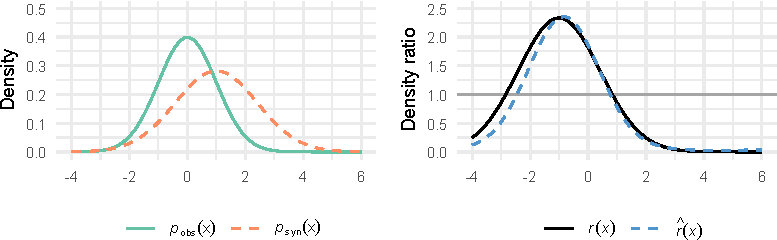
\includegraphics[width=1\textwidth,height=\textheight]{paper_files/figure-pdf/fig-dr-plot-1.pdf}

}

\caption{\label{fig-dr-plot}Example of the true and estimated density
ratio of two normal distributions with different means and variances
(i.e., \(\psyn(\bx) = N(0,1)\) and \(\pobs(\bx) = N(1,2)\)). The
function \(r(\bx) = \psyn(\bx)/\pobs(\bx)\) denotes the true density
ratio, the function \(\hat{r}(\bx)\) denotes an estimate of the density
ratio based on \(\nsyn = \nobs = 200\) samples from each distribution
obtained with unconstrained Least-Squares Importance Fitting (uLSIF).
Note that the density ratio is itself not a proper density.}

\end{figure}

\hypertarget{estimating-the-density-ratio}{%
\subsubsection{Estimating the density
ratio}\label{estimating-the-density-ratio}}

Over the past years, several methods for direct density ratio estimation
have been developed. A large class of these methods attempt to directly
minimize the error between the true density ratio \(r(\bx)\) and its
estimate \(\hat{r}(\bx)\). Following this approach, we define a loss
function \(\mathcal{L}(r(\bx), \hat{r}(\bx))\) that measures the
discrepancy between the true and estimated density ratio. To give an
example, consider the following loss based on the squared error
\begin{equation}\protect\hypertarget{eq-squared-error}{}{
\begin{aligned}
\mathcal{L}_S(r(\bx), \hat{r}(\bx)) &= 
\frac{1}{2} \int (\hat{r}(\bx) - r(\bx))^2 \pobs(\bx) \text{d}\bx \\
&= \frac{1}{2} \int \hat{r}(\bx)^2 \pobs(\bx) \text{d}\bx - 
\int \hat{r}(\bx) r(\bx) \pobs(\bx) \text{d}\bx + 
\frac{1}{2} \int r(\bx)^2 \pobs(\bx) \text{d}\bx.
\end{aligned}
}\label{eq-squared-error}\end{equation} The second term can be
rewritten, because the denominator in \(r(\bx)\) cancels with
\(\pobs(\bx)\), while the third term is a constant with respect to the
parameters in the density ratio model and can thus be ignored. Hence, we
are left with the following loss function to minimize
\begin{equation}\protect\hypertarget{eq-squared-error-loss}{}{
\mathcal{L}'_S (r(\bx), \hat{r}(\bx)) = \frac{1}{2} \int \hat{r}(\bx)^2 \pobs(\bx) \text{d}\bx - \int \hat{r}(\bx) \psyn(\bx) \text{d}\bx,
}\label{eq-squared-error-loss}\end{equation} which is termed least
squares importance fitting (LSIF) by Kanamori, Hido, and Sugiyama
(\protect\hyperlink{ref-kanamori_ulsif_2009}{2009}).

This approach can be straightforwardly generalized to a wide class of
loss functions that fall under the family of Bregman divergences (see
\protect\hyperlink{ref-sugiyama_bregman_2012}{Sugiyama, Suzuki, and
Kanamori 2012b}; \protect\hyperlink{ref-mohamed2017learning}{Mohamed and
Lakshminarayanan 2017}). Then, a general class of losses is encompassed
by the expression
\begin{equation}\protect\hypertarget{eq-bregman-loss}{}{
\mathcal{L}_f (r(\bx), \hat{r}(\bx)) =
\int \Big(
f(r(\bx)) - f(\hat{r}(\bx)) - f'(\hat{r}(\bx))(r(\bx) - \hat{r}(\bx))
\Big) \pobs(\bx) \text{d}\bx,
}\label{eq-bregman-loss}\end{equation} where \(f\) is a differentiable
and strictly convex function with derivative \(f'\). Then, ignoring the
terms independent of \(\hat{r}(\bx)\) and noting that
\(r(\bx)\pobs(\bx) = \psyn(\bx)\), we obtain the following objective
\begin{equation}\protect\hypertarget{eq-bregman-objective}{}{
\mathcal{L}'_f (r(\bx), \hat{r}(\bx)) = \int 
\Big( 
f'(\hat{r}(\bx)) \hat{r}(\bx) - f(\hat{r}(\bx))
\Big)  \pobs(\bx) \text{d}\bx
- \int f'(\hat{r}(\bx)) \psyn(\bx)
\text{d}\bx.
}\label{eq-bregman-objective}\end{equation} Minimizing this loss for
different functions \(f\) yields different estimators for the density
ratio, that focus on different regions of the density ratio.\footnote{It
  is easy to see that using \(f(x) = \frac{1}{2}(x-1)^2\) turns the
  Bregman divergence (Equation~\ref{eq-bregman-objective}) into the
  squared error (Equation~\ref{eq-squared-error-loss}).} Specifically,
some estimators place more emphasis on accurately modelling the regions
in which the true density ratio is large, but less emphasis on
accurately estimating the smaller density ratios, and vice versa (see
\protect\hyperlink{ref-sugiyama_bregman_2012}{Sugiyama, Suzuki, and
Kanamori 2012b}; \protect\hyperlink{ref-menon2016dreloss}{Menon and Ong
2016}). Importantly, Sugiyama, Suzuki, and Kanamori
(\protect\hyperlink{ref-sugiyama_bregman_2012}{2012b}) show that the
Bregman divergence minimization approach to density ratio estimation is
equivalent to estimating the \(f\)-divergence
(\protect\hyperlink{ref-ali_silvey_divergence_1966}{Ali and Silvey
1966}) between the synthetic and observed data distributions. Hence,
when estimating the density ratio, one implicitly estimates the
divergence between the synthetic and observed data distributions.

After defining a loss function, we need a model for the density ratio
function \(\hat{r}(\bx)\). There are many possibilities to specify this
model, but a common choice is to use a linear model for the density
ratio (e.g., \protect\hyperlink{ref-huang_kmm_2006}{Huang et al. 2006};
\protect\hyperlink{ref-kanamori_ulsif_2009}{Kanamori, Hido, and Sugiyama
2009}; \protect\hyperlink{ref-izbicki_dre_2014}{Izbicki, Lee, and
Schafer 2014}; \protect\hyperlink{ref-gruber2024overcoming}{Gruber et
al. 2024}). That is, we define the density ratio model as
\begin{equation}\protect\hypertarget{eq-dr-model}{}{
\hat{r}(\bx) = \boldsymbol{\varphi}(\bx) \boldsymbol{\theta},
}\label{eq-dr-model}\end{equation} where \(\boldsymbol{\varphi}(\bx)\)
is a basis function vector, that transforms the data from a
\(p\)-dimensional to a \(b\)-dimensional space, and
\(\boldsymbol{\theta}\) is a \(b\)-dimensional parameter vector.
Although the model is linear in its parameters, the density ratio itself
is typically a non-linear function of the data due to the basis
functions. The parameter vector \(\boldsymbol{\theta}\) is estimated to
minimize the discrepancy with the true density ratio using the loss
function \(\mathcal{L}(r(\bx), \hat{r}(\bx))\) in
Equation~\ref{eq-bregman-objective}.

Also for the basis functions, several specifications are possible,
ranging from an identity function
(\protect\hyperlink{ref-qin_inferences_1998}{Qin 1998}) to normalizing
flows (\protect\hyperlink{ref-choi_featurized_2021}{Choi, Liao, and
Ermon 2021}) or neural networks
(\protect\hyperlink{ref-tiao2018dre}{Tiao 2018};
\protect\hyperlink{ref-uehara2016generative}{Uehara et al. 2016}).
However, a commonly used basis function in the density ratio literature
is the Gaussian kernel function (e.g.,
\protect\hyperlink{ref-huang_kmm_2006}{Huang et al. 2006};
\protect\hyperlink{ref-sugiyama_kliep_2007}{Sugiyama et al. 2007};
\protect\hyperlink{ref-kanamori_ulsif_2009}{Kanamori, Hido, and Sugiyama
2009}; \protect\hyperlink{ref-liu_change_2013}{Liu et al. 2013};
\protect\hyperlink{ref-gruber2024overcoming}{Gruber et al. 2024}), which
conveniently allows to model the non-linear density ratio using models
that are linear in their parameters. The Gaussian kernel function is
defined as \[
\boldsymbol{\varphi}(\bx) = \mathcal{K}(\bx_i, \boldsymbol{c}_j) = 
\exp\left(
- \frac{\lVert\bx - \boldsymbol{c}_j \rVert^2}{2 \sigma^2}
\right),
\] where \(\boldsymbol{c}_j\) (\(j \in 1, \dots, J\)) denotes the
centers of the Gaussian kernel functions, and \(\sigma\) controls the
kernel width (i.e., it defines over which distance differences between
the observations and the centers are considered relevant; for more
information on kernel functions, see, e.g.,
\protect\hyperlink{ref-murphy_pmlintro_2022}{Murphy 2022}). The
appropriate width of the kernel can be determined using
cross-validation. The centers are typically sampled from the data (in
our case, the observed and synthetic data can both be used, but it is
also possible to solely use the synthetic samples).

After defining the model and the loss function, the density ratio can be
easily estimated. The \texttt{densityratio} package in R
(\protect\hyperlink{ref-densityratio}{Volker 2023}) provides an
implementation of commonly used loss functions with a Gaussian kernel
basis function. The package comes with an easy-to-use interface,
automatic cross-validation of hyperparameters and builds on \texttt{C++}
for fast computation. However, for increased flexibility with respect to
loss functions and basis functions, one could use classic optimization
techniques as gradient descent or (quasi-)Newton methods, for example as
implemented in the \texttt{optim} function in the statistical software
\texttt{R} (\protect\hyperlink{ref-R}{R Core Team 2023}). Both
approaches are briefly illustrated in Appendix \ref{sec-app-A} (TODO).

\hypertarget{evaluating-data-utility-with-the-density-ratio}{%
\subsubsection{Evaluating data utility with the density
ratio}\label{evaluating-data-utility-with-the-density-ratio}}

After estimating the density ratio, the information provided by the
density ratio can be summarized in a divergence measure, using the fact
that estimating the density ratio is equivalent to estimating the
\(f\)-divergence between the synthetic and observed data distributions
(\protect\hyperlink{ref-sugiyama_bregman_2012}{Sugiyama, Suzuki, and
Kanamori 2012b}). Accordingly, we can use the estimated density ratio
function to estimate an \(f\)-divergence between the observed and
synthetic data, and use this divergence measure as a utility measure for
the synthetic data. Although this divergence statistic is difficult to
interpret in an absolute sense, it can be used as a relative measure of
quality of the synthetic data. That is, for different synthetic data
sets, we can calculate the divergence to the observed data, and compare
these values to determine which synthetic data set is most similar to
the observed data. In a more formal way, the \(f\)-divergence gives rise
to a test statistic that can be used to test the null hypothesis that
the synthetic data is generated from the same distribution as the
observed data. The corresponding \(p\)-value can be calculated by
comparing the observed test statistic to the null distribution of test
statistics obtained using random permutations of the observed and
synthetic data (see, for example,
\protect\hyperlink{ref-sugiyama_lstst_2011}{Sugiyama et al. 2011};
\protect\hyperlink{ref-Wornowizki2016}{Wornowizki and Fried 2016};
\protect\hyperlink{ref-kanamori_divergence_2012}{Kanamori, Suzuki, and
Sugiyama 2012a}). Lastly, the density ratio function itself can be
plotted against individual variables or pairs of variables to discover
whether particular variables are particularly poorly captured in the
synthetic data. Each of these strategies can be readily executed using
the \texttt{densityratio} package in \texttt{R}
(\protect\hyperlink{ref-densityratio}{Volker 2023}), and will be further
illustrated in the upcoming sections.

\textbf{Ik twijfel nog een beetje over de volgende zaken, en voordat ik
alles ga zitten uitwerken hoor ik graag eerst jullie mening:}

\begin{enumerate}
\def\labelenumi{\arabic{enumi}.}
\item
  Ik heb nu het deel over regularisatie eruit gelaten, omdat ik vond dat
  het wat afleid van de main ideas, maar kan deze ook gewoon toevoegen
  aan Equation~\ref{eq-bregman-objective}. Het kan ook casual opgemerkt
  worden wanneer het daadwerkelijk gebruikt wordt. Wat vinden jullie?
\item
  Dimension reduction: ik was niet zo zeker hoe ik dit er direct moest
  bouwen, want effectief is het niet veel anders dan de huidige aanpak,
  alleen met een andere basis function (namelijk
  \(\phi(x) = \mathcal{K}(x_i^T U, c_j^T U)\)), waarbij U ook parameters
  heeft die geschat worden. Anyway, ik kan aan het eind een sectie maken
  met dat DRE nog steeds lastig kan zijn in hoge dimensies, en dat daar
  oplossingen voor zijn (bijvoorbeeld een LFDA-stap voor ulsif, of LHSS,
  of the spectral density ratio estimation methode (laatste twee zitten
  allebei in het package)). Het punt is vooral dat ik niet wil dat het
  teveel afleidt van het main punt, namelijk density ratio estimation,
  maar qua content zou het misschien een eigen sectie verdienen, ook
  omdat het niet direct enorm aansluit bij de twee secties hierboven.
\end{enumerate}

\begin{enumerate}
\def\labelenumi{\arabic{enumi}.}
\setcounter{enumi}{2}
\item
  Denken jullie dat dit een goede plek is om wat dieper in te gaan op
  mogelijke voordelen van density ratio estimation? Ik dacht dat na
  sectie 2.2.2 een voor de hand liggende plek zou zijn om hier wat
  dieper op in te gaan, en dan specifiek de volgende punten te benoemen:
  utility quantifications at every point in multivariate space, easy and
  flexible model specification through automatic model selection with
  cross-validation, potential for importance weighting, wellicht dan ook
  direct het punt van dimension reduction hierbij pakken.
\item
  Ik wil graag nog ergens iets zeggen over de relaties tussen density
  ratio estimation en de andere methodes (KL-divergence, pMSE), maar ik
  vraag me een beetje af of dat niet beter in de discussie kan.
\end{enumerate}

\begin{enumerate}
\def\labelenumi{\arabic{enumi}.}
\setcounter{enumi}{4}
\tightlist
\item
  Is dit echt de goede plaats om iets te zeggen over categorische
  variabelen? Deze kunnen namelijk gewoon geïncludeerd worden, maar met
  een Gaussian kernel wordt dat misschien een beetje awkward.
  Desalniettemin kan het prima, en kunnen we er ook voor kiezen om in de
  discussie te benoemen dat we een oplossing hebben gekozen, maar dat er
  ook andere opties zijn (bijv. andere kernels).
\end{enumerate}

\hypertarget{numerical-illustrations-simulation-studies}{%
\section{Numerical illustrations: Simulation
studies}\label{numerical-illustrations-simulation-studies}}

To evaluate the performance of density ratio estimation and compare it
to existing methods, we conduct a series of simulation studies. We
consider a variety of scenarios, including univariate and multivariate
models, varying correlations, number of variables, and sample sizes. To
perform density ratio estimation, we use unconstrained Least-Squares
Importance Fitting (uLSIF;
\protect\hyperlink{ref-kanamori_ulsif_2009}{Kanamori, Hido, and Sugiyama
2009}) as implemented in the \texttt{densityratio} package in \texttt{R}
(\protect\hyperlink{ref-densityratio}{Volker 2023}), because it fast and
has been shown to perform well in a variety of settings {[}ADD CITATIONS
{]}. We compare the performance of uLSIF to the performance of the
\(p\)-MSE as implemented in the \texttt{R}-package \texttt{synthpop}.

\hypertarget{univariate-simulations}{%
\subsection{Univariate simulations}\label{univariate-simulations}}

For the sake of illustrational clarity, we first evaluate the
performance of density ratio estimation in a univariate setting where
its performance can be evaluated using visualizations. In the
simulations, we generate data according to four data-generating
mechanisms, (1) a Laplace distribution, (2) a log-normal distribution,
(3) a location-scale \(t\)-distribution and (4) a normal distribution.
Subsequently, we approximate the true data generating mechanism using a
Gaussian model with the same mean and variance as the original data.
This setting is similar to situations that are commonly encountered in
the synthetic data field, in the sense that the true data generating
mechanism is unknown and needs to be approximated using a simpler
approximating model. The exact specifications of the data generating
mechanisms are as follows:

\begin{enumerate}
\def\labelenumi{\arabic{enumi}.}
\tightlist
\item
  Laplace distribution with location parameter \(\mu = 1\) and scale
  parameter \(b = 1\).
\item
  Log-normal distribution with log-mean parameter
  \(\mu_{\text{log}} = \log \{1/\sqrt{3} \}\) and log-standard deviation
  parameter \(\sigma_\text{log} = \sqrt{\log 3}\).
\item
  Location-scale \(t\)-distribution with location parameter \(\mu = 1\),
  scale parameter \(\tau^2 = 1\) and degrees of freedom \(\nu = 4\).
\item
  Normal distribution with mean \(\mu = 1\) and variance
  \(\sigma^2 = 2\).
\end{enumerate}

These data generating mechanisms are chosen such that they all have the
same population mean \(\mu = 1\) and variance \(\sigma^2 = 2\). The
approximating model is a Gaussian distribution with mean \(\mu = 1\) and
variance \(\sigma^2 = 2\). This distribution has the same mean and
variance, but differs in higher-order moments, except in the fourth
scenario. In the last simulation, we model the data generating mechanism
correctly to obtain some understanding into how density ratio estimation
behaves under a well-specified synthesis model. In all scenarios, we
generate \(500\) data sets with \(\nobs = 250\) observations from the
true data generating mechanism, and \(\nsyn = 250\) synthetic
observations from the approximating Gaussian model. The density ratio
model is estimated using uLSIF with a Gaussian kernel and an
\(L_2\)-regularization parameter. Both the kernel bandwidth and the
regularization parameter are selected using cross-validation, using the
default settings as implemented in the \texttt{densityratio} package.

\begin{figure}[t]

{\centering 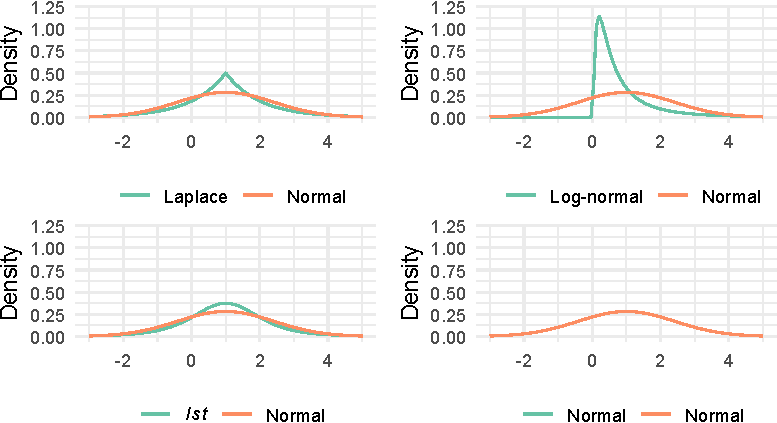
\includegraphics[width=1\textwidth,height=\textheight]{paper_files/figure-pdf/fig-densities-sim1-1.pdf}

}

\caption{\label{fig-densities-sim1}True and synthetic data densities for
the four simulations with Laplace, Log-normal, location-scale \(t\)- and
Normal densities. All data-generating mechanisms have the same mean
\(\mu = 1\) and variance \(\sigma^2 = 2\). Note that the true and
synthetic data density in the bottom right panel are completely
overlapping.}

\end{figure}

\begin{figure}[t]

{\centering 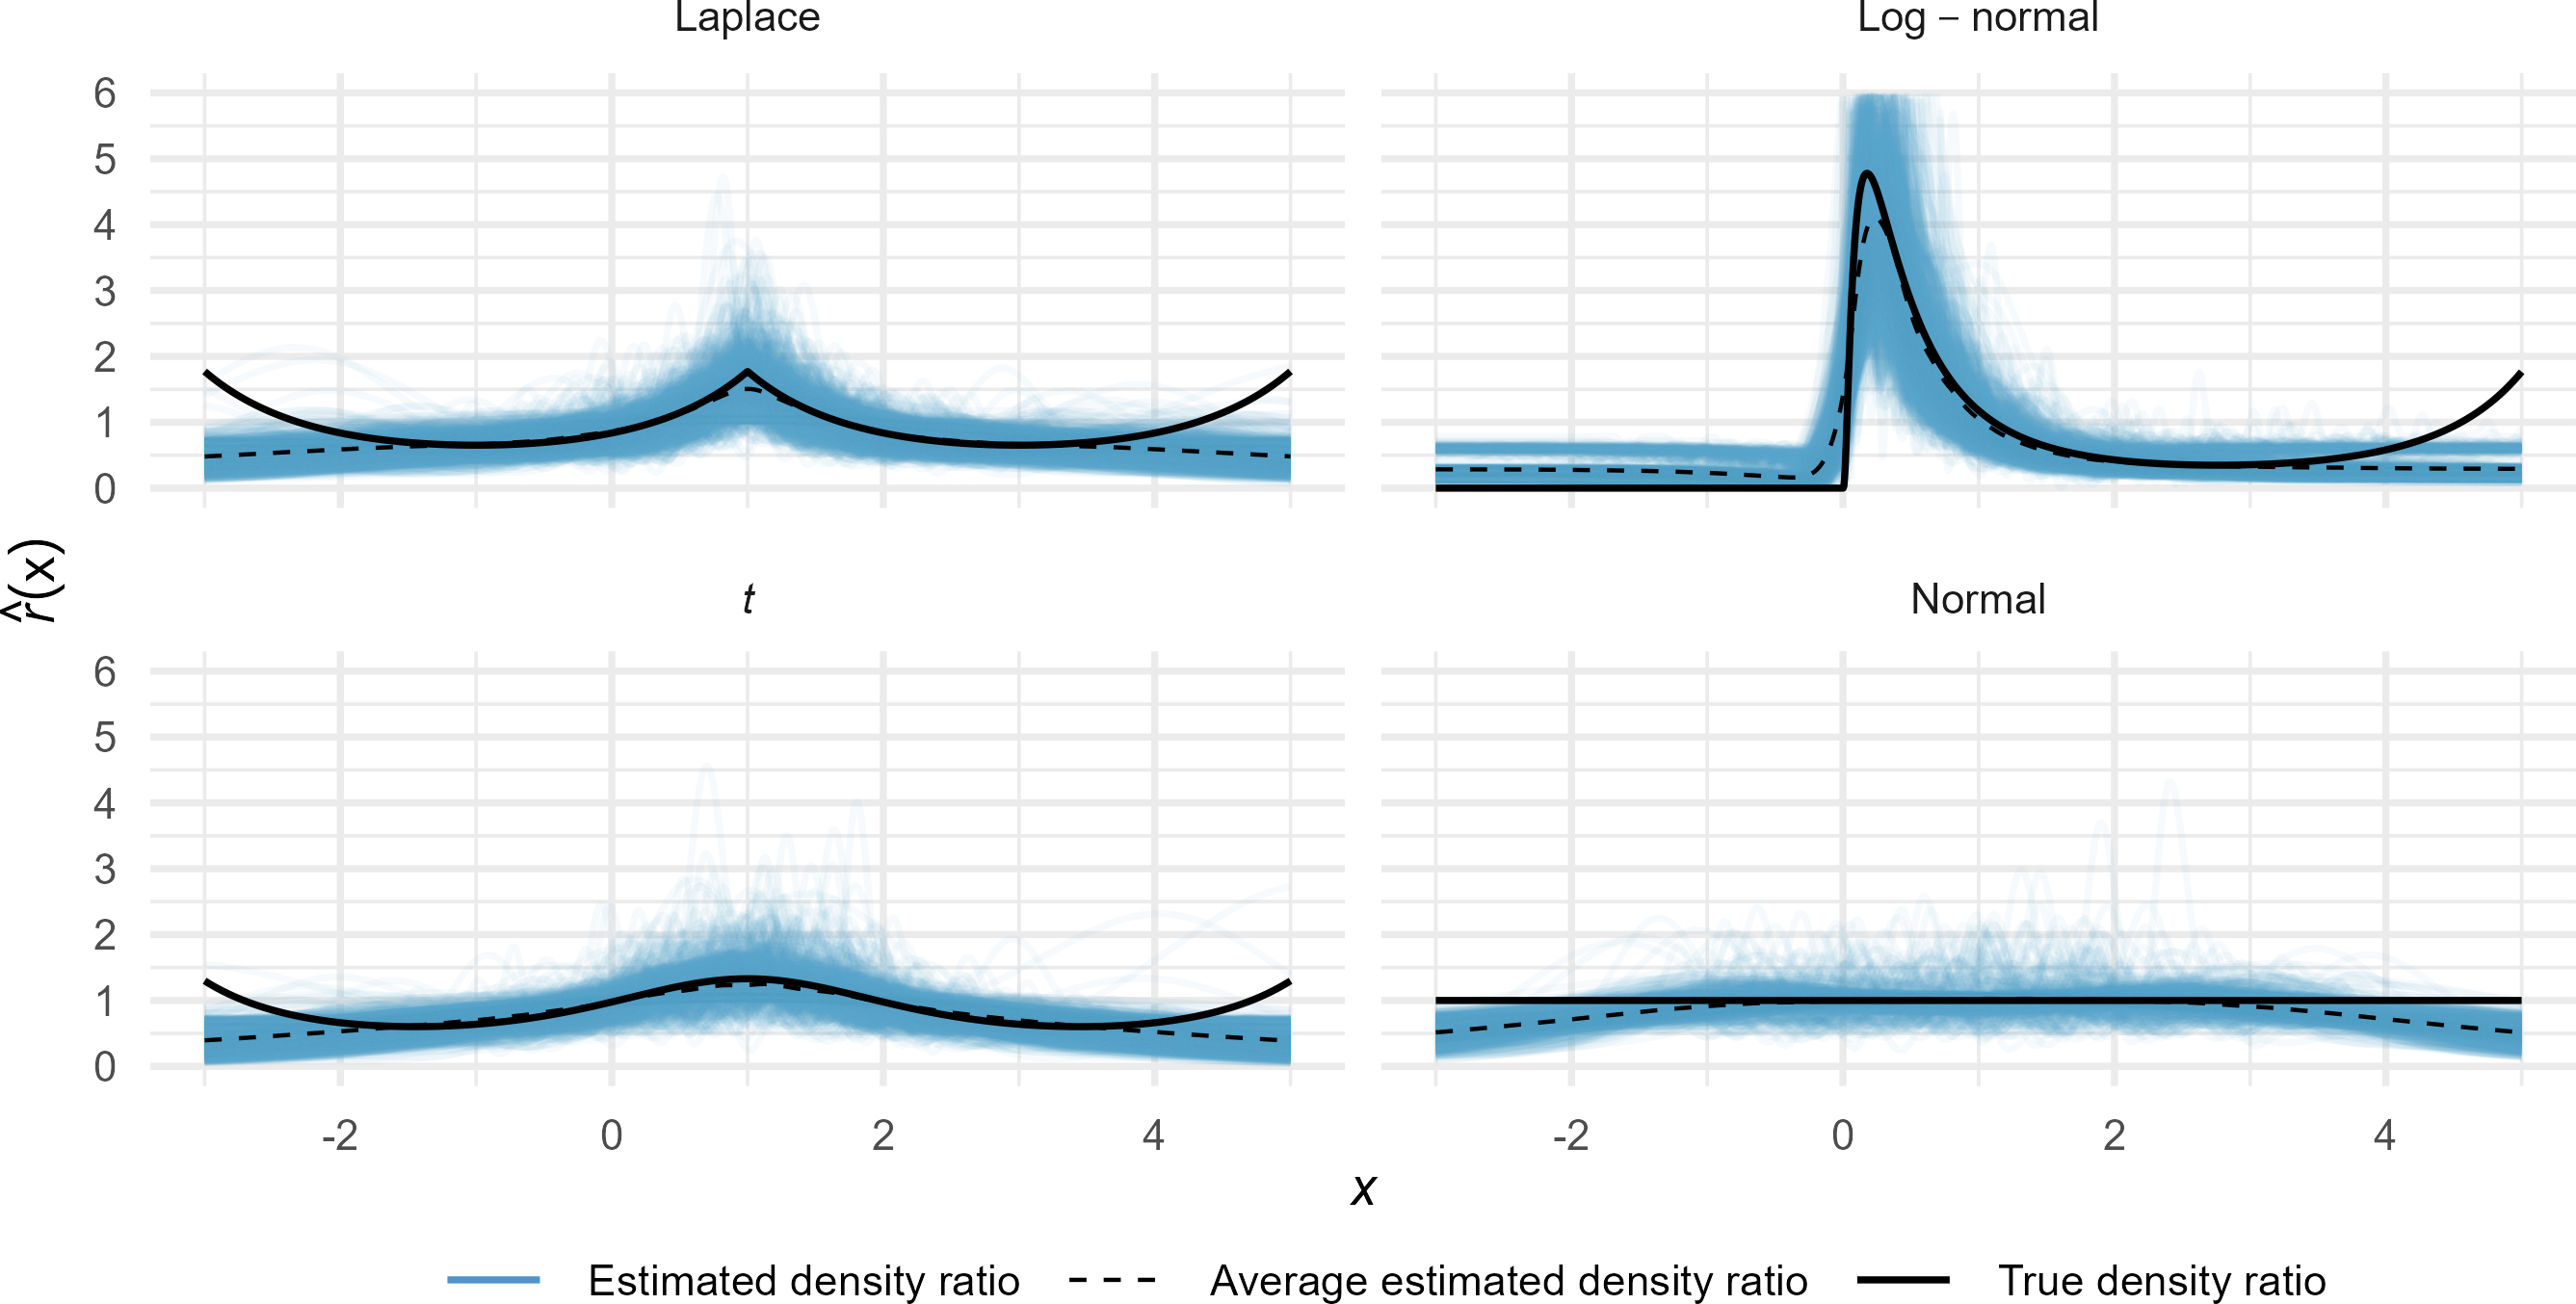
\includegraphics[width=1\textwidth,height=\textheight]{paper_files/figure-pdf/fig-sim1-results-1.pdf}

}

\caption{\label{fig-sim1-results}Estimated density ratios by
unconstrained least-squares importance fitting in four univariate
examples: A Laplace distribution, a log-normal distribution, a
location-scale \(t\)-distribution and a normal distribution, all
approximated by a normal distribution with the same mean and variance as
the sample from the true distribution.}

\end{figure}

TODO: Add interpretation of output; add significance tests and compare
with \(pMSE\) and kolmogorov-smirnov.

\hypertarget{multivariate-simulations}{%
\subsection{Multivariate simulations}\label{multivariate-simulations}}

TODO: Adjust section title

Currently, my plan is as follows, specify a (two/four) true data
generating mechanism: A multivariate normal distribution with a given
correlation structure, 7 and 17 variables each for two different sample
size (say n = 500 and n = 2000). Append the multivariate normal
distribution with three variables with a different distribution that
depend on the other variables through some non-linear function. Have
three synthetic data generating mechanisms, a simple multivariate normal
distribution with the same means and variances but zero covariances, a
model that uses a multivariate normal distribution with correlation
structure taken from the real data but misses the non-linear effects
(and marginal distributions of these variables), and a model that is
equivalent to the true model. Then, evaluate the quality of the
synthetic data sets using density ratio estimation and the \(pMSE\), and
see which of the two ranks the models correctly most of the time.

\hypertarget{application-synthetic-data-generation-for-the-u.s.-current-population-survey}{%
\section{Application: Synthetic data generation for the U.S. Current
Population
Survey}\label{application-synthetic-data-generation-for-the-u.s.-current-population-survey}}

ADD TEXT

\begin{figure}[t]

{\centering 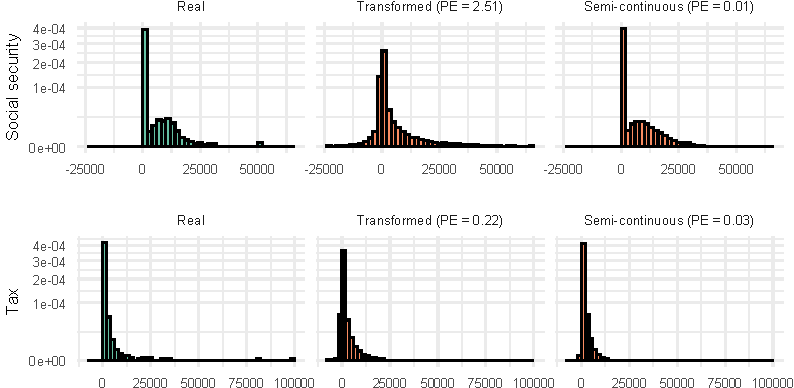
\includegraphics[width=1\textwidth,height=\textheight]{paper_files/figure-pdf/fig-application-distributions-1.pdf}

}

\caption{\label{fig-application-distributions}Real and synthetic data
distributions for the variables age, household income (income),
household property taxes (tax) and social security benefits (social
security) on a cubic root scale.}

\end{figure}

\begin{figure}[t]

{\centering 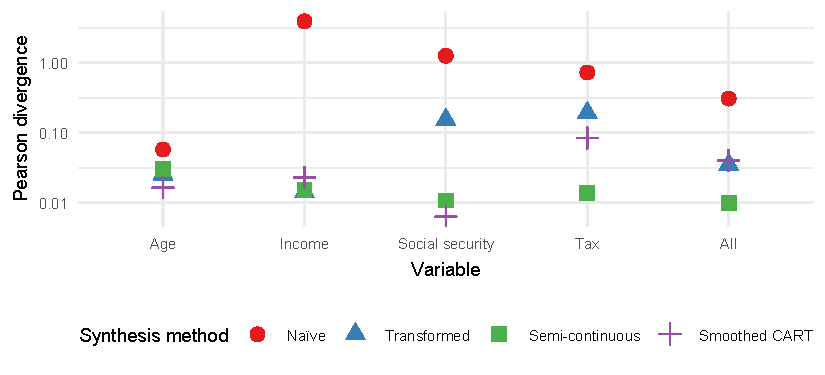
\includegraphics[width=1\textwidth,height=\textheight]{paper_files/figure-pdf/fig-application-pearson-div-1.pdf}

}

\caption{\label{fig-application-pearson-div}Pearson divergence estimates
after different synthesis strategies for the separate variables and the
synthetic data as a whole.}

\end{figure}

TODO: Expand example

High-dimensional density ratio estimation

Use density ratio values for weighted analysis

Incorporate point on individual data utility

\begin{itemize}
\tightlist
\item
  High dimensional example
\item
  Expansion of discussion points: empirical example with weighted
  analyses individual data utility
\end{itemize}

\hypertarget{discussion-and-conclusion}{%
\section{Discussion and conclusion}\label{discussion-and-conclusion}}

Adapt from previous version

\begin{itemize}
\tightlist
\item
  Privacy remark?
\item
  When does it not work?
\end{itemize}

Density ratios can be used directly to train generative models, see:
\href{https://arxiv.org/pdf/1610.03483}{Mohamed \& Lakshminarayanan
(2016)} and \href{https://arxiv.org/pdf/1610.02920.pdf}{Uehara, Sata,
Suzuki, Nakayama \& Matsuo (2016)}

Density ratio estimation is equivalent to class probability estimation
in classification problems, only differing in the loss function that is
employed (assuming the same model class is used for density ratio
estimation and classification). See
\href{https://proceedings.mlr.press/v48/menon16.pdf}{Menon \& Ong, 2016}

Logistic regression achieves the minimum asymptotic variance for
correctly specified models (Qin, Biometrika 1998), but is not reliable
for misspecified models (Kanamori, Suzuki, Sugiyama, IECE, 2010)

\hypertarget{references}{%
\section*{References}\label{references}}
\addcontentsline{toc}{section}{References}

\hypertarget{refs}{}
\begin{CSLReferences}{1}{0}
\leavevmode\vadjust pre{\hypertarget{ref-SIPP_Beta_2006}{}}%
Abowd, John M., Martha Stinson, and Gary Benedetto. 2006. {``Final
Report to the Social Security Administration on the {SIPP/SSA/IRS}
Public Use File Project.''} Longitudinal Employer-Household Dynamics
Program, U.S. Bureau of the Census, Washington, DC.
\url{https://ecommons.cornell.edu/bitstream/handle/1813/43929/SSAfinal.pdf?sequence=3\&isAllowed=y}.

\leavevmode\vadjust pre{\hypertarget{ref-ali_silvey_divergence_1966}{}}%
Ali, S. M., and S. D. Silvey. 1966. {``A General Class of Coefficients
of Divergence of One Distribution from Another.''} \emph{Journal of the
Royal Statistical Society. Series B (Methodological)} 28 (1): 131--42.
\url{https://doi.org/10.1111/j.2517-6161.1966.tb00626.x}.

\leavevmode\vadjust pre{\hypertarget{ref-atenas_open_2015}{}}%
Atenas, Javiera, Leo Havemann, and Ernesto Priego. 2015. {``Open Data as
Open Educational Resources: Towards Transversal Skills and Global
Citizenship.''} \emph{Open Praxis} 7 (4): 377--89.
\url{https://www.learntechlib.org/p/161986}.

\leavevmode\vadjust pre{\hypertarget{ref-Bowen_differentially_2021}{}}%
Bowen, Claire McKay, Fang Liu, and Bingyue Su. 2021. {``Differentially
Private Data Release via Statistical Election to Partition
Sequentially.''} \emph{METRON} 79 (1): 1--31.
\url{https://doi.org/10.1007/s40300-021-00201-0}.

\leavevmode\vadjust pre{\hypertarget{ref-choi_featurized_2021}{}}%
Choi, Kristy, Madeline Liao, and Stefano Ermon. 2021. {``Featurized
Density Ratio Estimation.''} In \emph{Proceedings of the Thirty-Seventh
Conference on Uncertainty in Artificial Intelligence}, edited by Cassio
de Campos and Marloes H. Maathuis, 161:172--82. Proceedings of Machine
Learning Research. PMLR.
\url{https://proceedings.mlr.press/v161/choi21a.html}.

\leavevmode\vadjust pre{\hypertarget{ref-crosas_automating_2015}{}}%
Crosas, Mercè, Gary King, James Honaker, and Latanya Sweeney. 2015.
{``Automating Open Science for Big Data.''} \emph{The ANNALS of the
American Academy of Political and Social Science} 659 (1): 260--73.
\url{https://doi.org/10.1177/0002716215570847}.

\leavevmode\vadjust pre{\hypertarget{ref-drechsler2011synthetic}{}}%
Drechsler, Jörg. 2011. \emph{Synthetic Datasets for Statistical
Disclosure Control: Theory and Implementation}. New York: Springer
Science \& Business Media.
\url{https://doi.org/10.1007/978-1-4614-0326-5}.

\leavevmode\vadjust pre{\hypertarget{ref-drechsler2012}{}}%
---------. 2012. {``New Data Dissemination Approaches in Old Europe
{\textendash} Synthetic Datasets for a German Establishment Survey.''}
\emph{Journal of Applied Statistics} 39 (2): 243--65.
\url{https://doi.org/10.1080/02664763.2011.584523}.

\leavevmode\vadjust pre{\hypertarget{ref-drechsler_utility_2022}{}}%
---------. 2022. {``Challenges in Measuring Utility for Fully Synthetic
Data.''} In \emph{Privacy in Statistical Databases}, edited by Josep
Domingo-Ferrer and Maryline Laurent, 220--33. Cham: Springer
International Publishing.
\url{https://doi.org/10.1007/978-3-031-13945-1_16}.

\leavevmode\vadjust pre{\hypertarget{ref-drechsler2023}{}}%
Drechsler, Jörg, and Anna-Carolina Haensch. 2023. {``30 Years of
Synthetic Data.''} \url{https://doi.org/10.48550/ARXIV.2304.02107}.

\leavevmode\vadjust pre{\hypertarget{ref-gdpr}{}}%
European Parliament, and Council of the European Union. 2016.
{``Regulation ({EU}) 2016/679 of the {European} {Parliament} and of the
{Council}. Of 27 {April} 2016 on the Protection of Natural Persons with
Regard to the Processing of Personal Data and on the Free Movement of
Such Data, and Repealing {Directive} 95/46/{EC} ({General} {Data}
{Protection} {Regulation}).''} OJ L 119, 4.5.2016, p. 1--88. May 4,
2016. \url{https://eur-lex.europa.eu/eli/reg/2016/679/oj}.

\leavevmode\vadjust pre{\hypertarget{ref-fpf_2017}{}}%
Future of Privacy Forum. 2017. {``Understanding Corporate Data Sharing
Decisions: Practices, Challenges, and Opportunities for Sharing
Corporate Data with Researchers.''}

\leavevmode\vadjust pre{\hypertarget{ref-gruber2024overcoming}{}}%
Gruber, Lukas, Markus Holzleitner, Johannes Lehner, Sepp Hochreiter, and
Werner Zellinger. 2024. {``Overcoming Saturation in Density Ratio
Estimation by Iterated Regularization.''}
\url{https://doi.org/10.48550/arXiv.2402.13891}.

\leavevmode\vadjust pre{\hypertarget{ref-hawala_synthetic_2008}{}}%
Hawala, Sam. 2008. \emph{Producing Partially Synthetic Data to Avoid
Disclosure}.
\url{http://www.asasrms.org/Proceedings/y2008/Files/301018.pdf}.

\leavevmode\vadjust pre{\hypertarget{ref-shohei_dre_outlier_2008}{}}%
Hido, Shohei, Yuta Tsuboi, Hisashi Kashima, Masashi Sugiyama, and
Takafumi Kanamori. 2008. {``Inlier-Based Outlier Detection via Direct
Density Ratio Estimation.''} In \emph{2008 Eighth IEEE International
Conference on Data Mining}, edited by Fosca Giannotti, Dimitrios
Gunopulos, Franco Turini, Carlo Zaniolo, Naren Ramakrishnan, and Xindong
Wu, 223--32. \url{https://doi.org/10.1109/ICDM.2008.49}.

\leavevmode\vadjust pre{\hypertarget{ref-hu_advancing_2024}{}}%
Hu, Jingchen, and Claire McKay Bowen. 2024. {``Advancing Microdata
Privacy Protection: A Review of Synthetic Data Methods.''} \emph{WIREs
Computational Statistics} 16 (1): e1636.
https://doi.org/\url{https://doi.org/10.1002/wics.1636}.

\leavevmode\vadjust pre{\hypertarget{ref-huang_kmm_2006}{}}%
Huang, Jiayuan, Alexander J. Smola, Arthur Gretton, Karsten M.
Borgwardt, and Bernhard Schölkopf. 2006. {``Correcting Sample Selection
Bias by Unlabeled Data.''} In \emph{Advances in Neural Information
Processing Systems}, edited by B. Schölkopf, J. Platt, and T. Hoffman.
Vol. 19. MIT Press.
\url{https://proceedings.neurips.cc/paper_files/paper/2006/file/a2186aa7c086b46ad4e8bf81e2a3a19b-Paper.pdf}.

\leavevmode\vadjust pre{\hypertarget{ref-hundepool_disclosure_2012}{}}%
Hundepool, Anco, Josep Domingo-Ferrer, Luisa Franconi, Sarah Giessing,
Eric Schulte Nordholt, Keith Spicer, and Peter-Paul De Wolf. 2012.
\emph{Statistical Disclosure Control}. John Wiley \& Sons.
\url{https://doi.org/10.1002/9781118348239}.

\leavevmode\vadjust pre{\hypertarget{ref-izbicki_dre_2014}{}}%
Izbicki, Rafael, Ann Lee, and Chad Schafer. 2014. {``{High-Dimensional
Density Ratio Estimation with Extensions to Approximate Likelihood
Computation}.''} In \emph{Proceedings of the Seventeenth International
Conference on Artificial Intelligence and Statistics}, edited by Samuel
Kaski and Jukka Corander, 33:420--29. Proceedings of Machine Learning
Research. Reykjavik, Iceland: PMLR.
\url{https://proceedings.mlr.press/v33/izbicki14.html}.

\leavevmode\vadjust pre{\hypertarget{ref-kanamori_ulsif_2009}{}}%
Kanamori, Takafumi, Shohei Hido, and Masashi Sugiyama. 2009. {``A
Least-Squares Approach to Direct Importance Estimation.''} \emph{Journal
of Machine Learning Research} 10 (48): 1391--1445.
\url{http://jmlr.org/papers/v10/kanamori09a.html}.

\leavevmode\vadjust pre{\hypertarget{ref-kanamori_divergence_2012}{}}%
Kanamori, Takafumi, Taiji Suzuki, and Masashi Sugiyama. 2012a. {``\(f\)
-Divergence Estimation and Two-Sample Homogeneity Test Under
Semiparametric Density-Ratio Models.''} \emph{IEEE Transactions on
Information Theory} 58 (2): 708--20.
\url{https://doi.org/10.1109/TIT.2011.2163380}.

\leavevmode\vadjust pre{\hypertarget{ref-Kanamori2012}{}}%
---------. 2012b. {``Statistical Analysis of Kernel-Based Least-Squares
Density-Ratio Estimation.''} \emph{Machine Learning} 86 (3): 335--67.
\url{https://doi.org/10.1007/s10994-011-5266-3}.

\leavevmode\vadjust pre{\hypertarget{ref-karr_utility_2006}{}}%
Karr, Alan F., Christine N. Kohnen, Anna Oganian, Jerome P. Reiter, and
Ashish P. Sanil. 2006. {``A Framework for Evaluating the Utility of Data
Altered to Protect Confidentiality.''} \emph{The American Statistician}
60 (3): 224--32. \url{https://doi.org/10.1198/000313006X124640}.

\leavevmode\vadjust pre{\hypertarget{ref-kim_classification_2021}{}}%
Kim, Ilmun, Aaditya Ramdas, Aarti Singh, and Larry Wasserman. 2021.
{``{Classification accuracy as a proxy for two-sample testing}.''}
\emph{The Annals of Statistics} 49 (1): 411--34.
\url{https://doi.org/10.1214/20-AOS1962}.

\leavevmode\vadjust pre{\hypertarget{ref-lazer_css_2009}{}}%
Lazer, David, Alex Pentland, Lada Adamic, Sinan Aral, Albert-László
Barabási, Devon Brewer, Nicholas Christakis, et al. 2009.
{``Computational Social Science.''} \emph{Science} 323 (5915): 721--23.
\url{https://doi.org/10.1126/science.1167742}.

\leavevmode\vadjust pre{\hypertarget{ref-little_statistical_1993}{}}%
Little, Roderick J. A. 1993. {``Statistical Analysis of Masked Data.''}
\emph{Journal of Official Statistics} 9 (2): 407--7.
\url{https://www.scb.se/contentassets/ca21efb41fee47d293bbee5bf7be7fb3/statistical-analysis-of-masked-data.pdf}.

\leavevmode\vadjust pre{\hypertarget{ref-liu_change_2013}{}}%
Liu, Song, Makoto Yamada, Nigel Collier, and Masashi Sugiyama. 2013.
{``Change-Point Detection in Time-Series Data by Relative Density-Ratio
Estimation.''} \emph{Neural Networks} 43: 72--83.
\url{https://doi.org/10.1016/j.neunet.2013.01.012}.

\leavevmode\vadjust pre{\hypertarget{ref-menon2016dreloss}{}}%
Menon, Aditya, and Cheng Soon Ong. 2016. {``Linking Losses for Density
Ratio and Class-Probability Estimation.''} In \emph{Proceedings of the
33rd International Conference on Machine Learning}, edited by Maria
Florina Balcan and Kilian Q. Weinberger, 48:304--13. Proceedings of
Machine Learning Research. New York, New York, USA: PMLR.
\url{https://proceedings.mlr.press/v48/menon16.html}.

\leavevmode\vadjust pre{\hypertarget{ref-mohamed2017learning}{}}%
Mohamed, Shakir, and Balaji Lakshminarayanan. 2017. {``Learning in
Implicit Generative Models.''}
\url{https://doi.org/10.48550/arXiv.1610.03483}.

\leavevmode\vadjust pre{\hypertarget{ref-murphy_pmlintro_2022}{}}%
Murphy, Kevin P. 2022. \emph{Probabilistic Machine Learning: An
Introduction}. MIT Press. \href{https://probml.ai}{probml.ai}.

\leavevmode\vadjust pre{\hypertarget{ref-newman_future_2012}{}}%
Newman, Greg, Andrea Wiggins, Alycia Crall, Eric Graham, Sarah Newman,
and Kevin Crowston. 2012. {``The Future of Citizen Science: Emerging
Technologies and Shifting Paradigms.''} \emph{Frontiers in Ecology and
the Environment} 10 (6): 298--304. \url{https://doi.org/10.1890/110294}.

\leavevmode\vadjust pre{\hypertarget{ref-obels_analysis_2020}{}}%
Obels, Pepijn, Daniël Lakens, Nicholas A. Coles, Jaroslav Gottfried, and
Seth A. Green. 2020. {``Analysis of Open Data and Computational
Reproducibility in Registered Reports in Psychology.''} \emph{Advances
in Methods and Practices in Psychological Science} 3 (2): 229--37.
\url{https://doi.org/10.1177/2515245920918872}.

\leavevmode\vadjust pre{\hypertarget{ref-obermeyer2019}{}}%
Obermeyer, Ziad, Brian Powers, Christine Vogeli, and Sendhil
Mullainathan. 2019. {``Dissecting Racial Bias in an Algorithm Used to
Manage the Health of Populations.''} \emph{Science} 366 (6464): 447--53.
\url{https://doi.org/10.1126/science.aax2342}.

\leavevmode\vadjust pre{\hypertarget{ref-qin_inferences_1998}{}}%
Qin, Jing. 1998. {``{Inferences for case-control and semiparametric
two-sample density ratio models}.''} \emph{Biometrika} 85 (3): 619--30.
\url{https://doi.org/10.1093/biomet/85.3.619}.

\leavevmode\vadjust pre{\hypertarget{ref-R}{}}%
R Core Team. 2023. \emph{R: A Language and Environment for Statistical
Computing}. Vienna, Austria: R Foundation for Statistical Computing.
\url{https://www.R-project.org/}.

\leavevmode\vadjust pre{\hypertarget{ref-raab2017guidelines}{}}%
Raab, Gillian M., Beata Nowok, and Chris Dibben. 2017. {``Guidelines for
Producing Useful Synthetic Data.''}
\url{https://arxiv.org/abs/1712.04078}.

\leavevmode\vadjust pre{\hypertarget{ref-raab2021assessing}{}}%
Raab, Gillian M, Beata Nowok, and Chris Dibben. 2021. {``Assessing,
Visualizing and Improving the Utility of Synthetic Data.''}
\url{https://doi.org/10.48550/arXiv.2109.12717}.

\leavevmode\vadjust pre{\hypertarget{ref-ramachandran_open_2021}{}}%
Ramachandran, Rahul, Kaylin Bugbee, and Kevin Murphy. 2021. {``From Open
Data to Open Science.''} \emph{Earth and Space Science} 8 (5):
e2020EA001562. \url{https://doi.org/10.1029/2020EA001562}.

\leavevmode\vadjust pre{\hypertarget{ref-reiter_releasing_2004}{}}%
Reiter, Jerome P. 2004. {``{Releasing Multiply Imputed, Synthetic Public
use Microdata: An Illustration and Empirical Study}.''} \emph{Journal of
the Royal Statistical Society Series A: Statistics in Society} 168 (1):
185--205. \url{https://doi.org/10.1111/j.1467-985X.2004.00343.x}.

\leavevmode\vadjust pre{\hypertarget{ref-rubin_statistical_1993}{}}%
Rubin, Donald B. 1993. {``Statistical Disclosure Limitation.''}
\emph{Journal of Official Statistics} 9 (2): 461--68.
\url{https://www.scb.se/contentassets/ca21efb41fee47d293bbee5bf7be7fb3/discussion-statistical-disclosure-limitation2.pdf}.

\leavevmode\vadjust pre{\hypertarget{ref-Scott1992}{}}%
Scott, David W. 1992. \emph{Multivariate Density Estimation: Theory,
Practice, and Visualization}. Wiley.
\url{https://doi.org/10.1002/9780470316849}.

\leavevmode\vadjust pre{\hypertarget{ref-snoke_utility_2018}{}}%
Snoke, Joshua, Gillian M. Raab, Beata Nowok, Chris Dibben, and
Aleksandra Slavkovic. 2018. {``General and Specific Utility Measures for
Synthetic Data.''} \emph{Journal of the Royal Statistical Society.
Series A (Statistics in Society)} 181 (3): pp. 663--688.
\url{https://doi.org/10.1111/rssa.12358}.

\leavevmode\vadjust pre{\hypertarget{ref-sugiyama_classification_2010}{}}%
Sugiyama, Masashi. 2010. {``Superfast-Trainable Multi-Class
Probabilistic Classifier by Least-Squares Posterior Fitting.''}
\emph{IEICE Transactions on Information and Systems} E93-D (10).
\url{https://doi.org/10.1587/transinf.E93.D.2690}.

\leavevmode\vadjust pre{\hypertarget{ref-sugiyama_kliep_2007}{}}%
Sugiyama, Masashi, Shinichi Nakajima, Hisashi Kashima, Paul Buenau, and
Motoaki Kawanabe. 2007. {``Direct Importance Estimation with Model
Selection and Its Application to Covariate Shift Adaptation.''} In
\emph{Advances in Neural Information Processing Systems}, edited by J.
Platt, D. Koller, Y. Singer, and S. Roweis. Vol. 20. Curran Associates,
Inc.
\url{https://proceedings.neurips.cc/paper_files/paper/2007/file/be83ab3ecd0db773eb2dc1b0a17836a1-Paper.pdf}.

\leavevmode\vadjust pre{\hypertarget{ref-sugiyama_lstst_2011}{}}%
Sugiyama, Masashi, Taiji Suzuki, Yuta Itoh, Takafumi Kanamori, and
Manabu Kimura. 2011. {``Least-Squares Two-Sample Test.''} \emph{Neural
Networks} 24 (7): 735--51.
\url{https://doi.org/10.1016/j.neunet.2011.04.003}.

\leavevmode\vadjust pre{\hypertarget{ref-sugiyama_suzuki_kanamori_2012}{}}%
Sugiyama, Masashi, Taiji Suzuki, and Takafumi Kanamori. 2012a.
\emph{Density Ratio Estimation in Machine Learning}. Cambridge
University Press. \url{https://doi.org/10.1017/CBO9781139035613}.

\leavevmode\vadjust pre{\hypertarget{ref-sugiyama_bregman_2012}{}}%
---------. 2012b. {``Density-Ratio Matching Under the Bregman
Divergence: A Unified Framework of Density-Ratio Estimation.''}
\emph{Annals of the Institute of Statistical Mathematics} 64 (5):
1009--44. \url{https://doi.org/10.1007/s10463-011-0343-8}.

\leavevmode\vadjust pre{\hypertarget{ref-sugiyama_conditional_2010}{}}%
Sugiyama, Masashi, Ichiro Takeuchi, Taiji Suzuki, Takafumi Kanamori,
Hirotaka Hachiya, and Daisuke Okanohara. 2010. {``Conditional Density
Estimation via Least-Squares Density Ratio Estimation.''} In
\emph{Proceedings of the Thirteenth International Conference on
Artificial Intelligence and Statistics}, edited by Yee Whye Teh and Mike
Titterington, 9:781--88. Proceedings of Machine Learning Research. Chia
Laguna Resort, Sardinia, Italy: PMLR.
\url{https://proceedings.mlr.press/v9/sugiyama10a.html}.

\leavevmode\vadjust pre{\hypertarget{ref-tiao2018dre}{}}%
Tiao, Louis C. 2018. {``{D}ensity {R}atio {E}stimation for {KL}
{D}ivergence {M}inimization Between {I}mplicit {D}istributions.''}
\emph{Tiao.io}.
\url{https://tiao.io/post/density-ratio-estimation-for-kl-divergence-minimization-between-implicit-distributions/}.

\leavevmode\vadjust pre{\hypertarget{ref-uehara2016generative}{}}%
Uehara, Masatoshi, Issei Sato, Masahiro Suzuki, Kotaro Nakayama, and
Yutaka Matsuo. 2016. {``Generative Adversarial Nets from a Density Ratio
Estimation Perspective.''}
\url{https://doi.org/10.48550/arXiv.1610.02920}.

\leavevmode\vadjust pre{\hypertarget{ref-vandewiel2023}{}}%
van de Wiel, Mark A., Gwenaël G. R. Leday, Jeroen Hoogland, Martijn W.
Heymans, Erik W. van Zwet, and Ailko H. Zwinderman. 2023. {``Think
Before You Shrink: Alternatives to Default Shrinkage Methods Can Improve
Prediction Accuracy, Calibration and Coverage.''}
\url{https://doi.org/10.48550/ARXIV.2301.09890}.

\leavevmode\vadjust pre{\hypertarget{ref-densityratio}{}}%
Volker, Thom Benjamin. 2023. {``Densityratio: Direct Estimation of the
Ratio of Densities of Two Groups of Observations.''}
\url{https://github.com/thomvolker/densityratio}.

\leavevmode\vadjust pre{\hypertarget{ref-willenborg_elements_2001}{}}%
Willenborg, Leon, and Ton De Waal. 2001. \emph{Elements of Statistical
Disclosure Control}. Springer Science \& Business Media.
\url{https://doi.org/10.1007/978-1-4613-0121-9}.

\leavevmode\vadjust pre{\hypertarget{ref-Woo_global_2009}{}}%
Woo, Mi-Ja, Jerome P. Reiter, Anna Oganian, and Alan F. Karr. 2009.
{``Global Measures of Data Utility for Microdata Masked for Disclosure
Limitation.''} \emph{Journal of Privacy and Confidentiality} 1 (1).
\url{https://doi.org/10.29012/jpc.v1i1.568}.

\leavevmode\vadjust pre{\hypertarget{ref-Wornowizki2016}{}}%
Wornowizki, Max, and Roland Fried. 2016. {``Two-Sample Homogeneity Tests
Based on Divergence Measures.''} \emph{Computational Statistics} 31 (1):
291--313. \url{https://doi.org/10.1007/s00180-015-0633-3}.

\leavevmode\vadjust pre{\hypertarget{ref-xu_ctgan_2019}{}}%
Xu, Lei, Maria Skoularidou, Alfredo Cuesta-Infante, and Kalyan
Veeramachaneni. 2019. \emph{Modeling Tabular Data Using Conditional
GAN}. Edited by H. Wallach, H. Larochelle, A. Beygelzimer, F.
dAlché-Buc, E. Fox, and R. Garnett. Vol. 32. Curran Associates, Inc.
\url{https://proceedings.neurips.cc/paper_files/paper/2019/file/254ed7d2de3b23ab10936522dd547b78-Paper.pdf}.

\leavevmode\vadjust pre{\hypertarget{ref-zettler2021}{}}%
Zettler, Ingo, Christoph Schild, Lau Lilleholt, Lara Kroencke, Till
Utesch, Morten Moshagen, Robert Böhm, Mitja D. Back, and Katharina
Geukes. 2021. {``The Role of Personality in COVID-19-Related
Perceptions, Evaluations, and Behaviors: Findings Across Five Samples,
Nine Traits, and 17 Criteria.''} \emph{Social Psychological and
Personality Science} 13 (1): 299--310.
\url{https://doi.org/10.1177/19485506211001680}.

\end{CSLReferences}

\setcounter{section}{0}
\renewcommand{\thesection}{\Alph{section}}

\setcounter{table}{0}
\renewcommand{\thetable}{A\arabic{table}}

\setcounter{figure}{0}
\renewcommand{\thefigure}{A\arabic{figure}}

\hypertarget{sec-app-A}{%
\section{\texorpdfstring{Density ratio estimation in
\texttt{R}}{Density ratio estimation in R}}\label{sec-app-A}}

TO DO

Small example of ulsif in \texttt{densityratio}

Do the same with \texttt{optim}

Do the same for a different loss function



\end{document}
